% coding:utf-8

%FOSAET, a LaTeX-Code for a electrical summary of basic electronics
%Copyright (C) 2013, Daniel Winz, Ervin Mazlagic

%This program is free software; you can redistribute it and/or
%modify it under the terms of the GNU General Public License
%as published by the Free Software Foundation; either version 2
%of the License, or (at your option) any later version.

%This program is distributed in the hope that it will be useful,
%but WITHOUT ANY WARRANTY; without even the implied warranty of
%MERCHANTABILITY or FITNESS FOR A PARTICULAR PURPOSE.  See the
%GNU General Public License for more details.
%----------------------------------------

\section{Zählpfeilsysteme}

\begin{figure}[h!]
	\centering
	\begin{subfigure}[b]{0.4\textwidth}
		\centering
		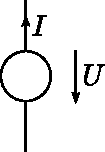
\includegraphics[scale=\schscale]{erzpfeilsys_sch.pdf}
		\caption{Erzeugerpfeilsystem}
		\label{sch:erzpfeilsys}
	\end{subfigure}
	\begin{subfigure}[b]{0.4\textwidth}
		\centering
		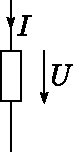
\includegraphics[scale=\schscale]{verbpfeilsys_sch.pdf}
		\caption{Verbraucherpfeilsystem}
		\label{sch:verbpfeilsys}
	\end{subfigure}
	\caption{Zählpfeilsysteme}
	\label{sch:pfeilsys}
\end{figure}

\subsection{Erzeugerpfeilsystem}
Zweipol wirk als Erzeuger, wenn das Produkt aus $U$ und $I$ positiv ist. Sonst wirkt er als Verbraucher. 

\subsection{Verbraucherpfeilsystem}
Zweipol wirk als Verbraucher, wenn das Produkt aus $U$ und $I$ positiv ist. Sonst wirkt er als Erzeuger. 
